\section{Iron---Orbital magnetization}
\label{sec19:IronOM}

\begin{itemize}
	\item Outline: {\it Calculate the orbital magnetization of ferromagnetic bcc Fe by Wannier interpolation.}
\end{itemize}

\begin{itemize}
	\item[1-6] These are the same steps performed for Ex.~\ref{sec17:IronSO} and Ex.~\ref{sec18:IronBerry}. Hence, they are not repeated here.

	\item {\it The orbital magnetization is computed as the BZ integral of the quantity $\mathbf{M}^{\mathrm{orb}}(\bfk)$ defined in Eq. (12.20)
of the User Guide.}

Below we report Eq. (11.20) from the User Guide, and the total orbital magnetization as the integral of $\mathbf{M}^{\mathrm{orb}}(\bfk)$ over the BZ
\begin{align}
\mathbf{M}^{\mathrm{orb}}(\bfk) & = \sum_{n}\frac{1}{2}f_{n\bfk}\;\mathrm{Im} \braket{\nabla_{\bfk}\unk \vert \times (H_\bfk + \epsilon_\bfk - 2\epsilon_{\mathrm{F}}) \vert \nabla_\bfk \unk}
\label{eq19.1} \\
\mathbf{M}^{\mathrm{orb}}_{\mathrm{tot}} & = V\int\,\frac{\diffk}{(2\pi)^3} \mathbf{M}^{\mathrm{orb}}(\bfk)
\label{eq19.2}
\end{align}

The two snippets below show the components of the total orbital magnetization computed according to Eq.~(\ref{eq19.2}), and the spin magnetisation from the DFT calculation respectively  
{\small
\begin{tcolorbox}[title=From Fe.wpout,sharp corners,boxrule=0.5pt]
\begin{verbatim}
 Properties calculated in module  b e r r y
 ------------------------------------------

   * Orbital magnetization
  
 Interpolation grid: 25 25 25


 Fermi energy (ev) =   12.628300


 M_orb (bohr magn/cell)        x          y          z
 ======================
    Local circulation :      0.0000    -0.0000     0.0935
 Itinerant circulation:      0.0000     0.0000    -0.0180
 --------------------------------------------------------
              Total   :      0.0000    -0.0000     0.0755

\end{verbatim}
\end{tcolorbox}
}

{\small
\begin{tcolorbox}[title=From scf.out,sharp corners,boxrule=0.5pt]
\begin{verbatim}
     total magnetization       =     0.00    -0.00    -2.22 Bohr mag/cell
     absolute magnetization    =     2.34 Bohr mag/cell
\end{verbatim}
\end{tcolorbox}

}

\item {\it Plot $\mathbf{M}^{\mathrm{orb}}(\bfk)$ along high-symmetry lines and compare the result with Fig.~2 of Ref.~\onlinecite{PhysRevB85}.}

Before comparing the result of our calculation with the result in Fig.~2 of Ref.~\onlinecite{PhysRevB85},  
we need to fix a unit-conversion problem in the python script {\tt Fe-bands+morb\_z.py}. In fact, the units of $\mathbf{M}^{\mathrm{orb}}(\bfk)$ are not Ry$\cdot\si{\angstrom}^2$ as stated in the python script but eV$\cdot\si{\angstrom}^2$ instead (as also stated in the User Guide). Moreover, in Ref.~\onlinecite{PhysRevB85} $\mathbf{M}^{\mathrm{orb}}(\bfk)$ is given in atomic units, i.e. Hartree$\cdot$bohr radii$^2$. In order to have a meaningful comparison we need to modify the python script accordingly. Open {\tt Fe-bands+morb\_z.py} and modify the following lines
{\tt
\begin{quote}
data = np.loadtxt('Fe-morb.dat')

x=data[:,0]

y=data[:,3]
\end{quote}
}

as 

{\tt
\begin{quote}
data = np.loadtxt('Fe-morb.dat')

x=data[:,0]

y=data[:,3] * 0.131234
\end{quote}
}
where $0.131234$ is the conversion factor from eV$\cdot\si{\angstrom}^2$ to a.u. We also need to modify the label for the y-axis from

\begin{quote}
\begin{verbatim}
	pl.ylabel(r'$M^{\rm{orb}}_z(\mathbf{k})$  [ Ry$\cdot\AA^2$ ]')
\end{verbatim}
\end{quote}

to

\begin{quote}
\begin{verbatim}
	pl.ylabel(r'$M^{\rm{orb}}_z(\mathbf{k})$  [ a.u. ]')
\end{verbatim}
\end{quote}

Now we can run the python script

{\tt
\begin{quote}
\$> python Fe-bands+morb\_z.py
\end{quote}
}

and look at the plot, here shown in \Fig{fig19.1}. 
The difference between the quantities in the two plot is roughly the $-\frac{1}{2}$ factor due to the two different definitions of $\mathbf{M}^{\mathrm{orb}}$.   
\begin{figure}[t!]
\centering
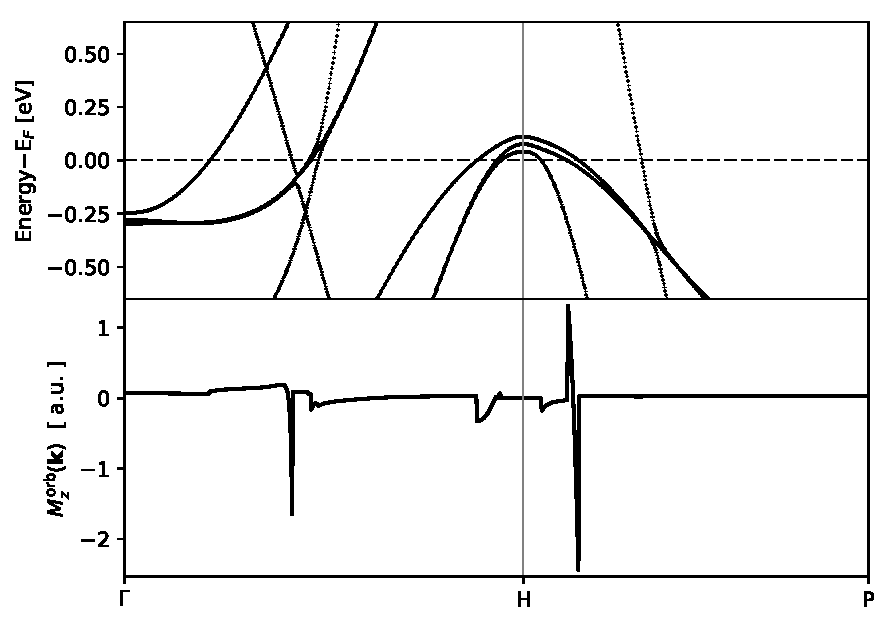
\includegraphics[width=0.6\columnwidth]{figure/example19/Fe-morb_z.pdf}
\caption{Plot of $\mathbf{M}^{\mathrm{orb}}(\bfk)$ calculated by Wannier
interpolation along the path $\Gamma$--H--P in the Brillouin zone.}\label{fig19.1}
\end{figure}

{\it Plot $\mathbf{M}^{\mathrm{orb}}(\bfk)$ together with the Fermi contours on the (010) BZ plane}

\begin{figure}[b!]
\centering
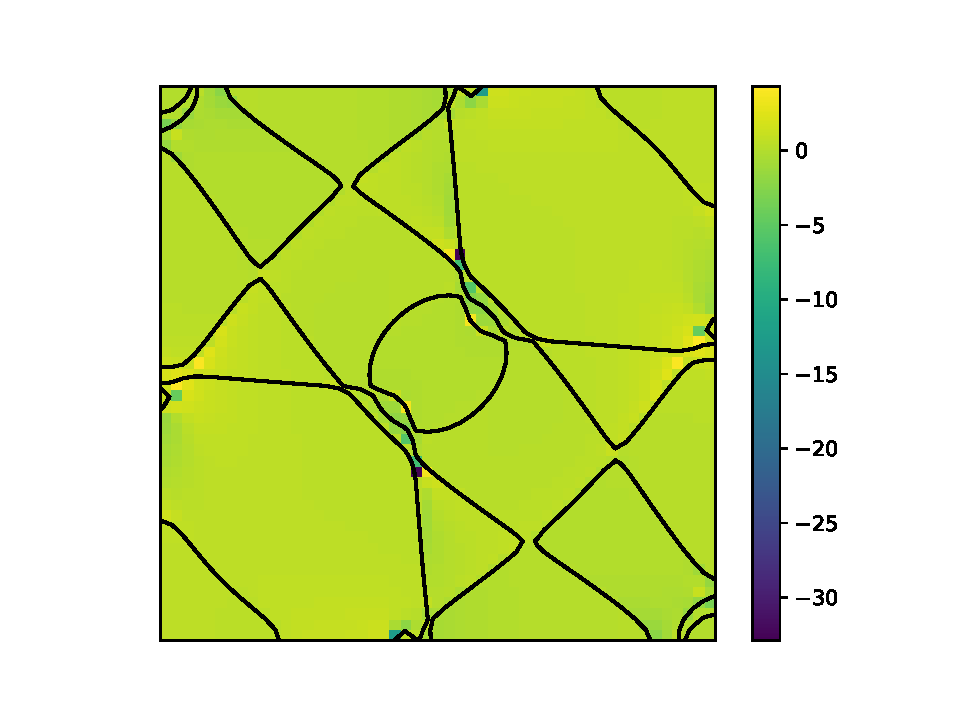
\includegraphics[width=0.7\columnwidth]{figure/example19/Fe-kslice-morb_z+fermi_lines.pdf}
\caption{Plot of $\mathbf{M}^{\mathrm{orb}}(\bfk)$ together with the Fermi contours on the (010) BZ plane}\label{fig19.3}
\end{figure}

\end{itemize}
